\section{DFP与BFGS}
\label{sec:qn-dfp-bfgs}

割线条件留下了很大的自由度。接下来要弄清：怎样用尽量小的对称修正满足它，同时让矩阵保持正定？答案是两个秩一项之和，改动的对象不同，就得到DFP和BFGS两种更新。

讨论一次更新时省略迭代上标：当前矩阵写作$\bm{B}$、$\bm{W}$，新矩阵写作$\bm{B}^{+}$、$\bm{W}^{+}$，位移和梯度差写作$\bm{s}$、$\bm{y}$，并记
\begin{equation}
 \rho=\frac{1}{\langle\bm{s},\bm{y}\rangle}.
 \label{eq:qn-rho}
\end{equation}

\paragraph{主要思想：秩二修正}
设新矩阵是旧矩阵加上两个对称秩一项：
\[
 \bm{B}^{+}=\bm{B}+a\bm{u}\bm{u}^\top+b\bm{v}\bm{v}^\top.
\]
代入割线条件$\bm{B}^{+}\bm{s}=\bm{y}$，得到
\[
 \bm{B}\bm{s}+a\langle\bm{u},\bm{s}\rangle\bm{u}+b\langle\bm{v},\bm{s}\rangle\bm{v}=\bm{y}.
\]

这个等式左边有三个向量，右边是$\bm{y}$。最直接的配法是让新增的一项产生$\bm{y}$，另一项抵消$\bm{B}\bm{s}$，也就是取$\bm{u}=\bm{y}$，$\bm{v}=\bm{B}\bm{s}$，并令
\[
 a\langle\bm{y},\bm{s}\rangle=1,\qquad b\,\bm{s}^\top\bm{B}\bm{s}=-1.
\]
由此得到\term{BFGS更新}（BFGS update）：
\begin{equation}
 \bm{B}^{+}=\bm{B}-\frac{\bm{B}\bm{s}\bm{s}^\top\bm{B}}{\bm{s}^\top\bm{B}\bm{s}}+\rho\,\bm{y}\bm{y}^\top.
 \label{eq:qn-bfgs-direct}
\end{equation}
名称取自Broyden、Fletcher、Goldfarb和Shanno四人。

更新的两项各做一件事。把旧矩阵减去第一项后的结果记为
\[
 \bm{P}=\bm{B}-\frac{\bm{B}\bm{s}\bm{s}^\top\bm{B}}{\bm{s}^\top\bm{B}\bm{s}}.
\]
它满足$\bm{P}\bm{s}=\bm{0}$，也就是把旧矩阵沿$\bm{s}$的曲率清空了。第二项把新测到的曲率填回去，因为$\rho\,\bm{y}\bm{y}^\top\bm{s}=\bm{y}$。

图~\ref{fig:qn-bfgs-strip}按贯穿例的第一次更新画出这个过程。旧矩阵的单位等值线是圆；清空沿$\bm{s}$的曲率之后，它变成沿$\bm{s}$无限延伸的带；加上测量项后，带又合拢成椭圆，形状已经向真实Hessian靠拢。

\begin{BookInlineFigure}
  \centering
  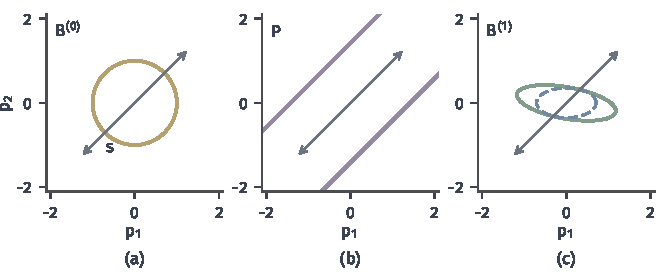
\includegraphics[width=112mm]{figures/05-optimization/02-smooth-optimization/matplotlib/qn-bfgs-strip/figure.pdf}
  \caption{贯穿例第一次BFGS更新的两步，曲线都是集合$\{\bm{p}:\bm{p}^\top\bm{M}\bm{p}=1\}$，箭头是$\bm{s}^{(0)}$所在的直线。(a)$\bm{M}=\bm{B}^{(0)}=\bm{I}$。(b)$\bm{M}=\bm{P}$，沿$\bm{s}$的曲率被清空，等值线变成平行的两条直线（紫）。(c)$\bm{M}=\bm{B}^{(1)}$（绿），加上测量项后重新合拢；蓝色虚线是真实Hessian的等值线。}
  \label{fig:qn-bfgs-strip}
\end{BookInlineFigure}

\paragraph{主要思想：对偶的DFP}
把同样的推导用在逆矩阵上。设$\bm{W}^{+}$是$\bm{W}$加上两个对称秩一项，代入割线条件~\eqref{eq:qn-secant-inverse}，取一项产生$\bm{s}$，另一项抵消$\bm{W}\bm{y}$，得到\term{DFP更新}（DFP update）：
\begin{equation}
 \bm{W}^{+}=\bm{W}-\frac{\bm{W}\bm{y}\bm{y}^\top\bm{W}}{\bm{y}^\top\bm{W}\bm{y}}+\rho\,\bm{s}\bm{s}^\top.
 \label{eq:qn-dfp-inverse}
\end{equation}
名称取自Davidon、Fletcher和Powell三人。对比式~\eqref{eq:qn-bfgs-direct}，两者互为对偶：在一个公式里交换$\bm{B}\leftrightarrow\bm{W}$、$\bm{s}\leftrightarrow\bm{y}$，就得到另一个。

实际计算只需要$\bm{W}$，方向~\eqref{eq:qn-direction}才不用解方程。DFP本来就是$\bm{W}$的公式，BFGS却要从$\bm{B}$翻译过来。下面的定理给出翻译的结果。

\begin{theorem}[BFGS的逆形式]
\label{thm:qn-bfgs-inverse}
设$\bm{B}\succ\bm{0}$，$\bm{W}=\bm{B}^{-1}$，$\bm{s}\neq\bm{0}$，$\langle\bm{s},\bm{y}\rangle>0$，并记$\bm{V}=\bm{I}-\rho\,\bm{y}\bm{s}^\top$。则式~\eqref{eq:qn-bfgs-direct}的$\bm{B}^{+}$可逆，其逆是
\begin{equation}
 \bm{W}^{+}=\bm{V}^\top\bm{W}\bm{V}+\rho\,\bm{s}\bm{s}^\top.
 \label{eq:qn-bfgs-inverse}
\end{equation}
\end{theorem}

\begin{proof}
只需验证$\bm{B}^{+}\bm{W}^{+}=\bm{I}$。先处理$\bm{B}^{+}\bm{V}^\top$。因为$\bm{V}^\top=\bm{I}-\rho\,\bm{s}\bm{y}^\top$，且$\bm{B}^{+}\bm{s}=\bm{y}$，所以
\[
 \bm{B}^{+}\bm{V}^\top=\bm{B}^{+}-\rho\,\bm{y}\bm{y}^\top=\bm{P}.
\]

再乘$\bm{W}$，由$\bm{B}\bm{W}=\bm{I}$，得到
\[
 \bm{P}\bm{W}=\bm{I}-\frac{\bm{B}\bm{s}\bm{s}^\top}{\bm{s}^\top\bm{B}\bm{s}}.
\]

接着由$\rho$的定义计算$\bm{s}^\top\bm{V}$：
\[
 \bm{s}^\top\bm{V}=\bm{s}^\top-\rho\langle\bm{s},\bm{y}\rangle\bm{s}^\top=\bm{0}^\top.
\]

所以右乘$\bm{V}$时第二项消失：
\[
 \bm{P}\bm{W}\bm{V}=\bm{V}.
\]

最后合并$\bm{W}^{+}$的两部分，并再用一次$\bm{B}^{+}\bm{s}=\bm{y}$：
\[
 \bm{B}^{+}\bm{W}^{+}=\bm{P}\bm{W}\bm{V}+\rho\,\bm{B}^{+}\bm{s}\bm{s}^\top=\bm{V}+\rho\,\bm{y}\bm{s}^\top=\bm{I}.
\]
方阵有右逆即可逆，定理得证。
\end{proof}

同样的公式也可以两次使用Sherman--Morrison公式得到，秩一修正求逆的公式可参考\BookChapterRef{chap:direct-linear-solvers}{卷二第12章“线性方程的直接求解”}。对偶地，DFP的直接形式是
\begin{equation}
 \bm{B}^{+}=\bm{V}\bm{B}\bm{V}^\top+\rho\,\bm{y}\bm{y}^\top.
 \label{eq:qn-dfp-direct}
\end{equation}

\paragraph{主要思想：新测量取代旧记忆}
逆形式~\eqref{eq:qn-bfgs-inverse}有一个清楚的解释。任取向量$\bm{z}$，令$a=\rho\langle\bm{s},\bm{z}\rangle$，由$\bm{V}$的定义，
\begin{equation}
 \bm{z}=a\,\bm{y}+\bm{V}\bm{z},\qquad\langle\bm{s},\bm{V}\bm{z}\rangle=0.
 \label{eq:qn-z-decomposition}
\end{equation}
也就是说，$\bm{z}$被拆成沿$\bm{y}$的部分和与$\bm{s}$正交的部分（这个拆分不是正交分解）。

把$\bm{W}^{+}$作用到$\bm{z}$上，得到
\[
 \bm{W}^{+}\bm{z}=a\,\bm{s}+\bm{V}^\top\bm{W}\bm{V}\bm{z}.
\]
沿$\bm{y}$的部分直接按测量结果换成$\bm{s}$，这正是割线条件；其余部分仍用旧矩阵$\bm{W}$处理，只是最后用$\bm{V}^\top$投影到$\bm{y}$的正交补上。图~\ref{fig:qn-bfgs-decomposition}画出了这个分解。

\begin{BookInlineFigure}
  \centering
  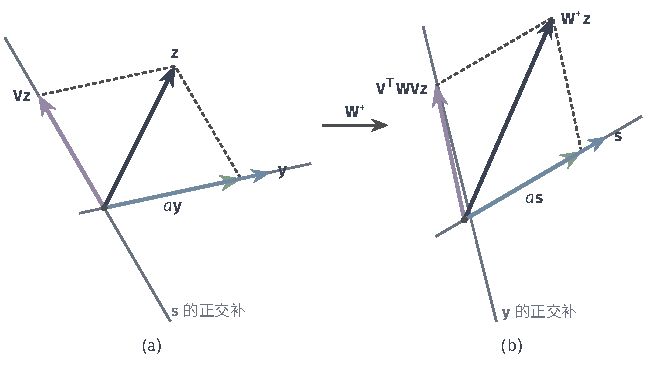
\includegraphics[width=108mm]{figures/05-optimization/02-smooth-optimization/tikz/qn-bfgs-decomposition/figure.pdf}
  \caption{BFGS逆更新对向量$\bm{z}$的作用，示意中旧矩阵取$\bm{W}=\bm{I}$。(a)$\bm{z}$沿$\bm{y}$与$\bm{s}$的正交补拆成两部分。(b)沿$\bm{y}$的部分$a\bm{y}$被换成$a\bm{s}$（绿），其余部分经旧矩阵后落在$\bm{y}$的正交补上（紫），两者相加得到$\bm{W}^{+}\bm{z}$。}
  \label{fig:qn-bfgs-decomposition}
\end{BookInlineFigure}

BFGS还有一个“改动最小”的刻画，它说明了在割线条件的整个解族中为什么选这一个。设$\bm{G}$是任意满足$\bm{G}\bm{s}=\bm{y}$的对称正定矩阵，例如$\bar{\bm{H}}$正定时的平均Hessian。在所有满足$\bm{W}=\bm{W}^\top$、$\bm{W}\bm{y}=\bm{s}$的矩阵中，BFGS的$\bm{W}^{+}$使加权距离$\lVert\bm{G}^{1/2}(\bm{W}-\bm{W}_{\mathrm{old}})\bm{G}^{1/2}\rVert_F$最小。

对偶地，DFP的$\bm{B}^{+}$在类似的约束下使$\lVert\bm{G}^{-1/2}(\bm{B}-\bm{B}_{\mathrm{old}})\bm{G}^{-1/2}\rVert_F$最小。证明需要把加权范数下的投影算出来，篇幅较长，读者可查阅\scite{math-nocedal2006numerical}。它的含义是：两种更新都尽量保留旧矩阵，只是一个在逆矩阵上度量改动，另一个在矩阵本身上度量改动。

\paragraph{曲率条件保证正定}
上一节说明曲率条件~\eqref{eq:qn-curvature-condition}是正定性的必要条件。现在证明，对BFGS和DFP它也是充分的。

\begin{theorem}[正定性的保持]
\label{thm:qn-positive-definite}
设$\bm{W}\succ\bm{0}$，$\bm{s}\neq\bm{0}$，$\bm{y}\neq\bm{0}$。则BFGS的$\bm{W}^{+}$与DFP的$\bm{W}^{+}$都正定，当且仅当$\langle\bm{s},\bm{y}\rangle>0$。
\end{theorem}

\begin{proof}
必要性：割线条件$\bm{W}^{+}\bm{y}=\bm{s}$与$\bm{y}$作内积，得到
\[
 \bm{y}^\top\bm{W}^{+}\bm{y}=\langle\bm{s},\bm{y}\rangle.
\]
若$\bm{W}^{+}\succ\bm{0}$，左边为正。

BFGS的充分性：对任意$\bm{z}\neq\bm{0}$，由式~\eqref{eq:qn-bfgs-inverse}，
\[
 \bm{z}^\top\bm{W}^{+}\bm{z}=(\bm{V}\bm{z})^\top\bm{W}(\bm{V}\bm{z})+\rho\langle\bm{s},\bm{z}\rangle^2.
\]
两项都非负。若第二项为零，则$\langle\bm{s},\bm{z}\rangle=0$，此时$\bm{V}\bm{z}=\bm{z}\neq\bm{0}$，第一项严格为正；所以和严格为正。

DFP的充分性：式~\eqref{eq:qn-dfp-direct}在结构上就是把式~\eqref{eq:qn-bfgs-inverse}中的$(\bm{W},\bm{s},\bm{y})$换成$(\bm{B},\bm{y},\bm{s})$，同样的论证给出$\bm{B}^{+}\succ\bm{0}$，因而$\bm{W}^{+}\succ\bm{0}$。
\end{proof}

\paragraph{Wolfe线搜索的作用}
剩下的问题是让曲率条件真的成立。第~\ref{sec:qn-secant}节留下的第二条Wolfe不等式正是为此准备的。记$\bm{s}=\alpha\bm{d}$，用第二条不等式，得到
\[
 \langle\bm{y},\bm{d}\rangle=\langle\bm{g}^{+},\bm{d}\rangle-\langle\bm{g},\bm{d}\rangle\geq(c_2-1)\langle\bm{g},\bm{d}\rangle.
\]
再乘以$\alpha>0$，由$c_2<1$和$\langle\bm{g},\bm{d}\rangle<0$，右端为正，于是
\begin{equation}
 \langle\bm{s},\bm{y}\rangle\geq\alpha(c_2-1)\langle\bm{g},\bm{d}\rangle>0.
 \label{eq:qn-wolfe-curvature}
\end{equation}
所以Wolfe线搜索对任意光滑目标都保证曲率条件，不需要目标是凸的。

只有充分下降条件是不够的。图~\ref{fig:qn-wolfe-curvature}取一维函数$\phi(\alpha)=f(\bm{x}+\alpha\bm{d})$，其导数为$\phi'(\alpha)=-1-1.5\alpha+\alpha^3$，它在起点附近向下弯。由$\bm{s}=\alpha\bm{d}$，曲率条件等价于$\phi'(\alpha)>\phi'(0)$。取$\alpha=0.5$，充分下降条件（$c_1=0.1$）成立，但
\[
 \phi'(0.5)=-1.625<-1=\phi'(0),
\]
曲率条件失败。取$c_2=0.5$时，第二条Wolfe不等式要求$\phi'(\alpha)\geq-0.5$，这把步长推到了$\alpha\geq1.37$，那里曲率的平均值已经为正。

\begin{BookInlineFigure}
  \centering
  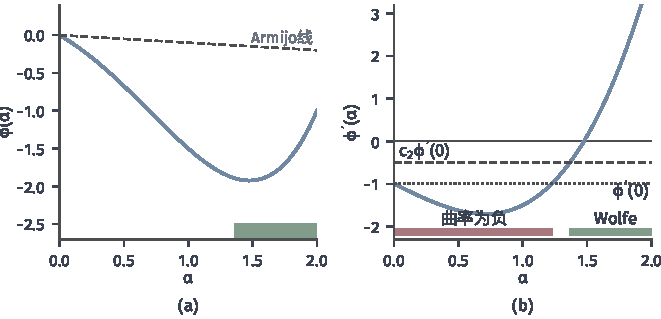
\includegraphics[width=112mm]{figures/05-optimization/02-smooth-optimization/matplotlib/qn-wolfe-curvature/figure.pdf}
  \caption{Wolfe条件怎样保证曲率条件，$\phi'(\alpha)=-1-1.5\alpha+\alpha^3$，$c_1=0.1$，$c_2=0.5$。(a)$\phi$（蓝）和充分下降的边界线（虚线），底部绿条是Wolfe条件的可接受步长。(b)$\phi'$（蓝）。红条上的步长满足$\phi'(\alpha)<\phi'(0)$，曲率条件失败；绿条上的步长满足$\phi'(\alpha)\geq c_2\phi'(0)$。}
  \label{fig:qn-wolfe-curvature}
\end{BookInlineFigure}

\paragraph{不用Wolfe时：跳过与阻尼}
有时线搜索只做回溯，或者步长由别的机制决定，曲率条件就可能不成立。这时有两种处理。

\textbf{跳过更新}：取小的正数$\varepsilon_{\mathrm{c}}$（如$10^{-8}$），当
\begin{equation}
 \langle\bm{s},\bm{y}\rangle\leq\varepsilon_{\mathrm{c}}\lVert\bm{s}\rVert_2\lVert\bm{y}\rVert_2
 \label{eq:qn-skip-rule}
\end{equation}
时令$\bm{W}^{+}=\bm{W}$。它保持正定，代价是这一次测量被扔掉。

\textbf{阻尼更新}：不扔掉测量，而是把$\bm{y}$与$\bm{B}\bm{s}$混合，使混合后的向量满足曲率要求。记曲率比
\[
 \tau=\frac{\langle\bm{s},\bm{y}\rangle}{\bm{s}^\top\bm{B}\bm{s}},
\]
再取
\begin{equation}
 \theta=\begin{cases}1,&\tau\geq0.2,\\\dfrac{0.8}{1-\tau},&\tau<0.2,\end{cases}\qquad
 \bm{r}=\theta\bm{y}+(1-\theta)\bm{B}\bm{s},
 \label{eq:qn-damping}
\end{equation}
再用$\bm{r}$代替$\bm{y}$代入式~\eqref{eq:qn-bfgs-direct}。

这样处理后$\tau<0.2$时的曲率比正好是$0.2$，因为
\[
 \frac{\langle\bm{s},\bm{r}\rangle}{\bm{s}^\top\bm{B}\bm{s}}=\theta\tau+1-\theta=1-\theta(1-\tau)=0.2.
\]
曲率比大于零，由定理~\ref{thm:qn-positive-definite}，$\bm{B}^{+}$正定。

用第~\ref{sec:qn-secant}节的不定例子算一次。取$\bm{B}=\bm{I}$，$\bm{s}=(1,2)^\top$，$\bm{y}=(2,-2)^\top$，则$\bm{s}^\top\bm{B}\bm{s}=5$，$\tau=-0.4$，于是
\[
 \theta=\frac{0.8}{1.4}=\frac47,\qquad
 \bm{r}=\frac47(2,-2)^\top+\frac37(1,2)^\top=\Bigl(\frac{11}{7},-\frac27\Bigr)^\top.
\]
验算：$\langle\bm{s},\bm{r}\rangle=11/7-4/7=1=0.2\times5$。图~\ref{fig:qn-damping}是$\theta$和修正前后曲率比的变化。

要注意阻尼放弃了什么：新矩阵满足$\bm{B}^{+}\bm{s}=\bm{r}$，而不再满足原来的割线条件。下表比较这三种机制。

\begin{BookInlineTable}
  \centering
  \begin{tabular}{lll}
    \toprule
    机制 & 曲率条件 & 代价\\
    \midrule
    Wolfe线搜索 & 由线搜索保证 & 可能多几次函数和梯度计算\\
    跳过更新 & 不成立时不更新 & 丢掉这次测量\\
    阻尼更新 & 由混合后的$\bm{r}$保证 & 放弃原来的割线条件\\
    \bottomrule
  \end{tabular}
  \caption{保持正定性的三种机制。}
  \label{tab:qn-curvature-mechanisms}
\end{BookInlineTable}

\begin{BookInlineFigure}
  \centering
  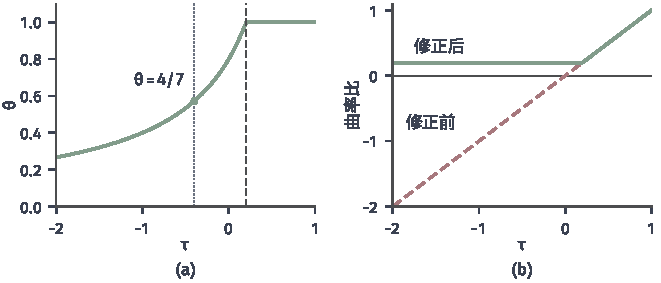
\includegraphics[width=112mm]{figures/05-optimization/02-smooth-optimization/matplotlib/qn-damping/figure.pdf}
  \caption{阻尼更新。(a)式~\eqref{eq:qn-damping}中的混合系数$\theta$随曲率比$\tau$的变化，虚线是阈值$\tau=0.2$，绿点是例中的$\tau=-0.4$，$\theta=4/7$。(b)修正前（红虚线）与修正后（绿）的曲率比，修正后不低于$0.2$。}
  \label{fig:qn-damping}
\end{BookInlineFigure}

\paragraph{计算过程}
下面用贯穿例~\eqref{eq:qn-running-example}完整走一遍BFGS，步长取精确线搜索，它在二次目标上满足Wolfe条件。

\needspace{6\baselineskip}
\paragraph{变量}
\begin{itemize}
 \item $\bm{x}^{(t)}\in\mathbb{R}^{n}$：当前迭代点；$\bm{g}^{(t)}\in\mathbb{R}^{n}$：当前梯度。
 \item $\bm{W}^{(t)}\in\mathbb{R}^{n\times n}$：对称正定的逆曲率近似。
 \item $\bm{d}^{(t)}$、$\alpha^{(t)}$：方向与步长。
 \item $\bm{s}^{(t)}$、$\bm{y}^{(t)}\in\mathbb{R}^{n}$、$\rho^{(t)}$：位移、梯度差与$1/\langle\bm{s}^{(t)},\bm{y}^{(t)}\rangle$。
\end{itemize}

\paragraph{初始化}
选起点$\bm{x}^{(0)}$和对称正定的$\bm{W}^{(0)}$，通常取单位矩阵的倍数，并计算$\bm{g}^{(0)}$。例中初始数据是
\[
 \bm{x}^{(0)}=(4,1)^\top,\qquad\bm{W}^{(0)}=\bm{I},\qquad\bm{g}^{(0)}=(8,8)^\top.
\]

\paragraph{每轮更新}
对$t=0,1,\ldots$依次执行下面的步骤，当$\lVert\bm{g}^{(t)}\rVert_2\leq\varepsilon$时停止。

\begin{enumerate}
\item 由式~\eqref{eq:qn-direction}计算方向$\bm{d}^{(t)}=-\bm{W}^{(t)}\bm{g}^{(t)}$。例中第一轮$\bm{d}^{(0)}=(-8,-8)^\top$。

\item 沿$\bm{d}^{(t)}$做满足式~\eqref{eq:qn-wolfe}的线搜索，优先试$\alpha=1$。例中用精确线搜索，第一轮的步长是
\[
 \alpha^{(0)}=\frac15.
\]

\item 更新迭代点并计算新梯度。例中第一轮得到
\[
 \bm{x}^{(1)}=(2.4,-0.6)^\top,\qquad\bm{g}^{(1)}=(4.8,-4.8)^\top.
\]

\item 由式~\eqref{eq:qn-s-y}计算$\bm{s}^{(t)}$、$\bm{y}^{(t)}$和$\rho^{(t)}$，并检查曲率条件。例中第一轮的$\bm{s}^{(0)}$、$\bm{y}^{(0)}$由式~\eqref{eq:qn-running-pair}给出，且
\[
 \langle\bm{s}^{(0)},\bm{y}^{(0)}\rangle=25.6,\qquad\rho^{(0)}=\frac{1}{25.6}.
\]

\item 用$\bm{s}^{(t)}$、$\bm{y}^{(t)}$、$\rho^{(t)}$构成定理~\ref{thm:qn-bfgs-inverse}中的$\bm{V}$，由式~\eqref{eq:qn-bfgs-inverse}更新$\bm{W}^{(t+1)}$。例中第一轮的两个中间量是
\[
 \bm{V}=\begin{bmatrix}0.8&-0.2\\-0.8&0.2\end{bmatrix},\qquad
 \rho^{(0)}\bm{s}^{(0)}\bigl(\bm{s}^{(0)}\bigr)^\top=\begin{bmatrix}0.1&0.1\\0.1&0.1\end{bmatrix}.
\]
由此得到
\[
 \bm{W}^{(1)}=\bm{V}^\top\bm{V}+\rho^{(0)}\bm{s}^{(0)}\bigl(\bm{s}^{(0)}\bigr)^\top
 =\begin{bmatrix}1.38&-0.22\\-0.22&0.18\end{bmatrix}.
\]
\end{enumerate}

$\bm{W}^{(1)}$的逆是
\[
 \bm{B}^{(1)}=\begin{bmatrix}0.9&1.1\\1.1&6.9\end{bmatrix},
\]
即族~\eqref{eq:qn-secant-family}中$a=0.9$的成员。验算割线条件，$\bm{W}^{(1)}\bm{y}^{(0)}$算出来确实是$(-1.6,-1.6)^\top$，也就是$\bm{s}^{(0)}$。

第二轮按同样的步骤进行。方向和精确步长是
\[
 \bm{d}^{(1)}=-\bm{W}^{(1)}\bm{g}^{(1)}=(-7.68,1.92)^\top,\qquad\alpha^{(1)}=\frac{46.08}{147.456}=\frac{5}{16}.
\]

于是迭代点到达
\[
 \bm{x}^{(2)}=\bm{x}^{(1)}+\alpha^{(1)}\bm{d}^{(1)}=(0,0)^\top,\qquad\bm{g}^{(2)}=\bm{0}.
\]
梯度为零，迭代结束。

为了看矩阵学到了什么，再做一次更新。这时有
\[
 \bm{s}^{(1)}=(-2.4,0.6)^\top,\qquad\bm{y}^{(1)}=(-4.8,4.8)^\top,\qquad\rho^{(1)}=\frac{1}{14.4}.
\]

由式~\eqref{eq:qn-bfgs-inverse}得到
\[
 \bm{W}^{(2)}=\begin{bmatrix}0.5&0\\0&0.125\end{bmatrix}=\bm{A}^{-1}.
\]
最终得到解$\bm{x}^{(2)}=\bm{0}$，而且两次测量之后逆曲率近似恰好等于真实Hessian的逆。图~\ref{fig:qn-bfgs-path}展示了路径和矩阵的变化。

\begin{BookInlineFigure}
  \centering
  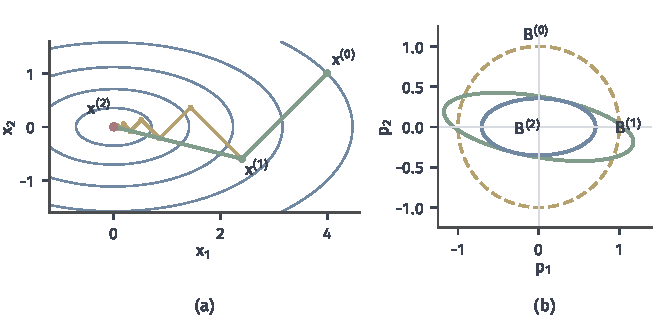
\includegraphics[width=112mm]{figures/05-optimization/02-smooth-optimization/matplotlib/qn-bfgs-path/figure.pdf}
  \caption{贯穿例上的BFGS。(a)蓝线是$f(\bm{x})=x_1^2+4x_2^2$的等高线，绿线是BFGS（$\bm{W}^{(0)}=\bm{I}$，精确线搜索）的两步，黄线是相同起点的最速下降。(b)集合$\{\bm{p}:\bm{p}^\top\bm{B}^{(t)}\bm{p}=1\}$，从圆（黄虚线）经过倾斜的椭圆（绿）变成真实Hessian的等值线（蓝）。}
  \label{fig:qn-bfgs-path}
\end{BookInlineFigure}

这不是巧合。在正定二次目标上使用精确线搜索时，BFGS产生的方向两两关于Hessian共轭，至多$n$步到达最优解，并且$\bm{W}^{(n)}=\bm{A}^{-1}$；第二次更新也没有破坏第一次的测量，例中可以验算$\bm{W}^{(2)}\bm{y}^{(0)}=\bm{s}^{(0)}$。证明用对步数的归纳法，篇幅较长，读者可查阅\scite{math-nocedal2006numerical}。这个结论依赖精确线搜索和二次目标，一般目标上不成立。

\paragraph{DFP与BFGS的对比}
用同一个例子算DFP。第一轮的$\bm{s}^{(0)}$、$\bm{y}^{(0)}$相同，由式~\eqref{eq:qn-dfp-inverse}得到
\[
 \bm{W}^{(1)}_{\mathrm{DFP}}=\frac{1}{170}\begin{bmatrix}177&-23\\-23&27\end{bmatrix}.
\]
它的逆是族~\eqref{eq:qn-secant-family}中$a=1.08$的成员。

矩阵不同，第二轮的方向却平行，$\bm{d}^{(1)}_{\mathrm{DFP}}$约为$(-5.647,1.412)^\top$，正好是BFGS方向的$0.735$倍。原因在于精确线搜索使$\langle\bm{g}^{(1)},\bm{s}^{(0)}\rangle=0$，再由割线条件和$\bm{d}^{(1)}=-\bm{W}^{(1)}\bm{g}^{(1)}$，得到
\[
 \langle\bm{y}^{(0)},\bm{d}^{(1)}\rangle=-\langle\bm{W}^{(1)}\bm{y}^{(0)},\bm{g}^{(1)}\rangle=-\langle\bm{s}^{(0)},\bm{g}^{(1)}\rangle=0.
\]
二维时这确定了方向。两种方法在这个例子上走过完全相同的点。

一旦线搜索不精确，差别就显现出来。图~\ref{fig:qn-dfp-bfgs-scaling}在一个$10$维强凸目标上比较两者，线搜索都满足强Wolfe条件。初始矩阵取$\bm{I}$时，两者都在约$20$步内收敛。

把初始矩阵缩小为$10^{-3}\bm{I}$，相当于矩阵$\bm{B}^{(0)}$的曲率估计过大，BFGS用$74$步恢复，DFP在$300$步后梯度大小仍约为$3.9$。这种从错误的曲率估计中恢复的能力称为自校正。第~\ref{sec:qn-convergence}节会用一个势函数解释BFGS的自校正，那个论证对DFP不适用。这就是实践中通常用BFGS而不用DFP的原因。

\begin{BookInlineFigure}
  \centering
  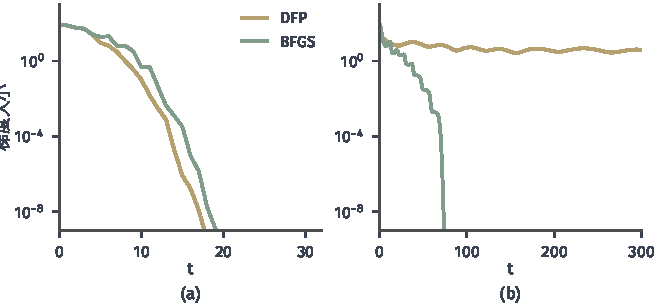
\includegraphics[width=112mm]{figures/05-optimization/02-smooth-optimization/matplotlib/qn-dfp-bfgs-scaling/figure.pdf}
  \caption{BFGS（绿）与DFP（黄）的梯度大小随迭代的变化。目标是$10$维强凸函数$\sum_i(\tfrac12c_iz_i^2+\ln\cosh z_i)$，其中$\bm{z}=\bm{Q}\bm{x}$，$\bm{Q}$是固定的正交矩阵，$c_i$在$[0.1,100]$上对数等距；线搜索为强Wolfe条件，$c_1=10^{-4}$，$c_2=0.9$。(a)$\bm{W}^{(0)}=\bm{I}$。(b)$\bm{W}^{(0)}=10^{-3}\bm{I}$，注意横轴范围不同。}
  \label{fig:qn-dfp-bfgs-scaling}
\end{BookInlineFigure}
